\section{Results}
The results consist of the following plots:
\begin{itemize}
	\item Enrichment SWU
	\item Reprocessing Waste (\gls{FP} \& \gls{MA} for scenario 1,2. Only \gls{FP} for scenario 3)
	\item Number of Reactors
	\item Net Installed Capacity
	\item Waste from Reactors that are not reprocessed (Over the Reprocessing Plant throughput)
	\item Reprocessed Uranium Stockpile
	\item Total Unused Tailings
	\item Fuel Usage
\end{itemize}
		
		
\subsection{Halt Reprocessing at 2020}

\begin{figure}
	\includegraphics[width=\linewidth]{./images/stoprep_2020/power_plot.png}
	\caption{Net Installed Capacity vs time}
	\label{fig:reprocess_capacity}
\end{figure}

\begin{figure}
	\includegraphics[width=\linewidth]{./images/stoprep_2020/Enrichment1_SWU.png}
	\caption{SWU vs time}
	\label{fig:reprocess_swu}
\end{figure}

\begin{figure}
	\includegraphics[width=\linewidth]{./images/stoprep_2020/total_fuel.png}
	\caption{Total Fuel Usage vs time}
	\label{fig:reprocess_fuel}
\end{figure}

\begin{figure}
	\includegraphics[width=\linewidth]{./images/stoprep_2020/FP_MA_total_Waste.png}
	\caption{Reprocessing Waste vs time}
	\label{fig:reprocess_rep_waste}
\end{figure}

\begin{figure}
	\includegraphics[width=\linewidth]{./images/stoprep_2020/Reactor_total_Waste.png}
	\caption{Total Spent Fuel Mass vs time}
	\label{fig:reprocess_reactor_waste}
\end{figure}

\begin{figure}
	\includegraphics[width=\linewidth]{./images/stoprep_2020/Separations_Total_Stockpile.png}
	\caption{Reprocessed Uranium Stockpile vs Time}
	\label{fig:reprocess_fuel}
\end{figure}

\begin{figure}
	\includegraphics[width=\linewidth]{./images/stoprep_2020/Tails_total_Waste.png}
	\caption{Leftover Tails vs Time}
	\label{fig:reprocess_tails}
\end{figure}


\subsection{Continue Reprocessing with \gls{MOX}}

\begin{figure}
	\includegraphics[width=\linewidth]{./images/reprocess/power_plot.png}
	\caption{Net Installed Capacity vs time}
	\label{fig:reprocess_capacity}
\end{figure}

\begin{figure}
	\includegraphics[width=\linewidth]{./images/reprocess/Enrichment1_SWU.png}
	\caption{SWU vs time}
	\label{fig:reprocess_swu}
\end{figure}

\begin{figure}
	\includegraphics[width=\linewidth]{./images/reprocess/total_fuel.png}
	\caption{Total Fuel Usage vs time}
	\label{fig:reprocess_fuel}
\end{figure}

\begin{figure}
	\includegraphics[width=\linewidth]{./images/reprocess/FP_MA_total_Waste.png}
	\caption{Reprocessing Waste vs time}
	\label{fig:reprocess_rep_waste}
\end{figure}

\begin{figure}
	\includegraphics[width=\linewidth]{./images/reprocess/Reactor_total_Waste.png}
	\caption{Total Spent Fuel Mass vs time}
	\label{fig:reprocess_reactor_waste}
\end{figure}

\begin{figure}
	\includegraphics[width=\linewidth]{./images/reprocess/Separations_Total_Stockpile.png}
	\caption{Reprocessed Uranium Stockpile vs Time}
	\label{fig:reprocess_fuel}
\end{figure}

\begin{figure}
	\includegraphics[width=\linewidth]{./images/reprocess/Tails_total_Waste.png}
	\caption{Leftover Tails vs Time}
	\label{fig:reprocess_tails}
\end{figure}

\subsection{Continuous Recycle with \gls{SFR}s}